\documentclass[a4paper,11pt,titlepage]{scrbook}
\usepackage[utf8]{inputenc}
\usepackage[spanish]{babel}

%\usepackage{titlesec}
%\usepackage{palatino} %usar fot palatino en vez de times roman

%\decimalpoint %revisar
%\usepackage{dcolumn} %revisat
%\newcolumntype{.}{D{.}{\esperiod}{-1}}
%\makeatletter
%\addto\shorthandsspanish{\let\esperiod\es@period@code}
%\makeatother


%\usepackage[chapter]{algorithm}
%\RequirePackage{verbatim}
%\RequirePackage[Glenn]{fncychap}
\usepackage{fancyhdr}
\usepackage{graphicx}
\usepackage{afterpage}
\usepackage{longtable}
\usepackage{xcolor}
\definecolor{portada}{RGB}{239,206,53}
\definecolor{base}{RGB}{35,31,32}
\usepackage{pdfpages}
\usepackage[acronym]{glossaries}
\usepackage{acronym}
\usepackage{breakcites}

\renewcommand{\glossaryname}{Glosario}
\renewcommand{\acronymname}{Acrónimos}

%Instrucciones para poder escribir código y mostrarlo de manera elegante:
\definecolor{gray97}{gray}{.97}
\definecolor{gray75}{gray}{.75}
\definecolor{gray45}{gray}{.45}
\definecolor{gray30}{gray}{.94}

\usepackage{listings}
\lstset{ frame=Ltb,
framerule=0pt,
aboveskip=0.5cm,
framextopmargin=3pt,
framexbottommargin=3pt,
framexleftmargin=0.4cm,
framesep=0pt,
rulesep=.4pt,
backgroundcolor=\color{gray97},
rulesepcolor=\color{black},
%
stringstyle=\ttfamily,
showstringspaces = false,
basicstyle=\small\ttfamily,
commentstyle=\color{gray45},
keywordstyle=\bfseries,
%
numbers=left,
numbersep=15pt,
numberstyle=\tiny,
numberfirstline = false,
breaklines=true,
literate={á}{{\'a}}1 {Á}{{\'A}}1 {é}{{\'e}}1 {É}{{\'e}}1 {í}{{\'i}}1  {Í}{{\'I}}1  {ó}{{\'o}}1  {Ó}{{\'O}}1  {ú}{{\'u}}1  {Ú}{{\'U}}1  {Ñ}{{\~N}}1 {ñ}{{\~n}}1 ,
}



% minimizar fragmentado de listados
\lstnewenvironment{listing}[1][]
   {\lstset{#1}\pagebreak[0]}{\pagebreak[0]}

\lstdefinestyle{Consola}
   {basicstyle=\scriptsize\bf\ttfamily,
    backgroundcolor=\color{gray30},
    frame=single,
    numbers=none
   }
\lstdefinestyle{C}
	{basicstyle=\scriptsize,
	frame=single,
	language=C,
	numbers=left
	}
\lstdefinestyle{CodigoC++}
        {basicstyle=\small,
	frame=single,
	backgroundcolor=\color{gray30},
	language=C++,
	numbers=left
 	}
\lstdefinestyle{PHP}
	{basicstyle=\scriptsize,
%        {basicstyle=\small,
	frame=single,
	language=PHP,
	numbers=left
	}
	



% ********************************************************************
% Información sobre el TFG. Comentar lo que NO se desee añadir y sustituir con la información correcta.
% ********************************************************************
\newcommand{\myTitle}{Título del Trabajo de Fin de Grado}
\newcommand{\mySubtitle}{Subtítulo del proyecto}
\newcommand{\myDegree}{Grado en Ingeniería Multimedia}
\newcommand{\myName}{José Luis Muñoz Periñán (alumno)}
\newcommand{\myProf}{Nombre Apellido1 Apellido2 (tutor1)}
\newcommand{\myOtherProf}{Nombre Apellido1 Apellido2 (tutor2)}
\newcommand{\myFaculty}{Escuela Politécnica Superior de la Universidad de Alicante}
\newcommand{\myFacultyShort}{EPS UA}
\newcommand{\depTutorOne}{Departamento del tutor}
\newcommand{\depTutorTwo}{Departamento del cotutor}


\newcommand{\myUni}{\protect{Universidad de Alicante}}
\newcommand{\myLocation}{Alicante}
\newcommand{\myTime}{\today}
%\newcommand{\myVersion}{Version 0.1}

\newcommand{\logoGrado}{imagenes/logoim.jpg}
\newcommand{\logoFacultad}{imagenes/logoeps.jpg}
\newcommand{\logoUniversidad}{imagenes/logoua.jpg}

\usepackage{url}

% Definición de comandos que me son útiles:
%\renewcommand{\indexname}{Índice alfabético}
%\renewcommand{\glossaryname}{Glosario}

\pagestyle{fancy}
\fancyhf{}
\fancyhead[LO]{\leftmark}
\fancyhead[RE]{\rightmark}
\fancyhead[RO,LE]{\textbf{\thepage}}
\renewcommand{\chaptermark}[1]{\markboth{\textbf{#1}}{}}
\renewcommand{\sectionmark}[1]{\markright{\textbf{\thesection. #1}}}


\setlength{\headheight}{1.5\headheight}

\newcommand{\HRule}{\rule{\linewidth}{0.5mm}}
%Definimos los tipos teorema, ejemplo y definición podremos usar estos tipos
%simplemente poniendo \begin{teorema} \end{teorema} ...
\newtheorem{teorema}{Teorema}[chapter]
\newtheorem{ejemplo}{Ejemplo}[chapter]
\newtheorem{definicion}{Definición}[chapter]
 
\newcommand{\bigrule}{\titlerule[0.5mm]}


%Para conseguir que en las páginas en blanco no ponga cabeceras
\makeatletter
\def\clearpage{%
  \ifvmode
    \ifnum \@dbltopnum =\m@ne
      \ifdim \pagetotal <\topskip
        \hbox{}
      \fi
    \fi
  \fi
  \newpage
  \thispagestyle{empty}
  \write\m@ne{}
  \vbox{}
  \penalty -\@Mi
}
\makeatother

\usepackage[pdfborder={000}]{hyperref} %referencia
\hypersetup{
pdfauthor = {\myName (email (en) ua (punto) es)},
pdftitle = {\myTitle},
pdfsubject = {},
pdfkeywords = {palabra_clave1, palabra_clave2, palabra_clave3, ...},
pdfcreator = {LaTeX con el paquete ....},
pdfproducer = {pdflatex}
}
%AQUI COMIENZA LA LISTA DE FICHEROS A INCLUIR


\begin{document}
\renewcommand{\listtablename}{Índice de tablas} %para sustituir la palabra cuadro por tabla
\renewcommand{\tablename}{Tabla}
\renewcommand{\lstlistingname}{Listado}
\renewcommand{\lstlistlistingname}{Índice de \lstlistingname s}

\frontmatter
\begin{titlepage}

\newlength{\centeroffset}
\setlength{\centeroffset}{-0.5\oddsidemargin}
\addtolength{\centeroffset}{0.5\evensidemargin}
\thispagestyle{empty}
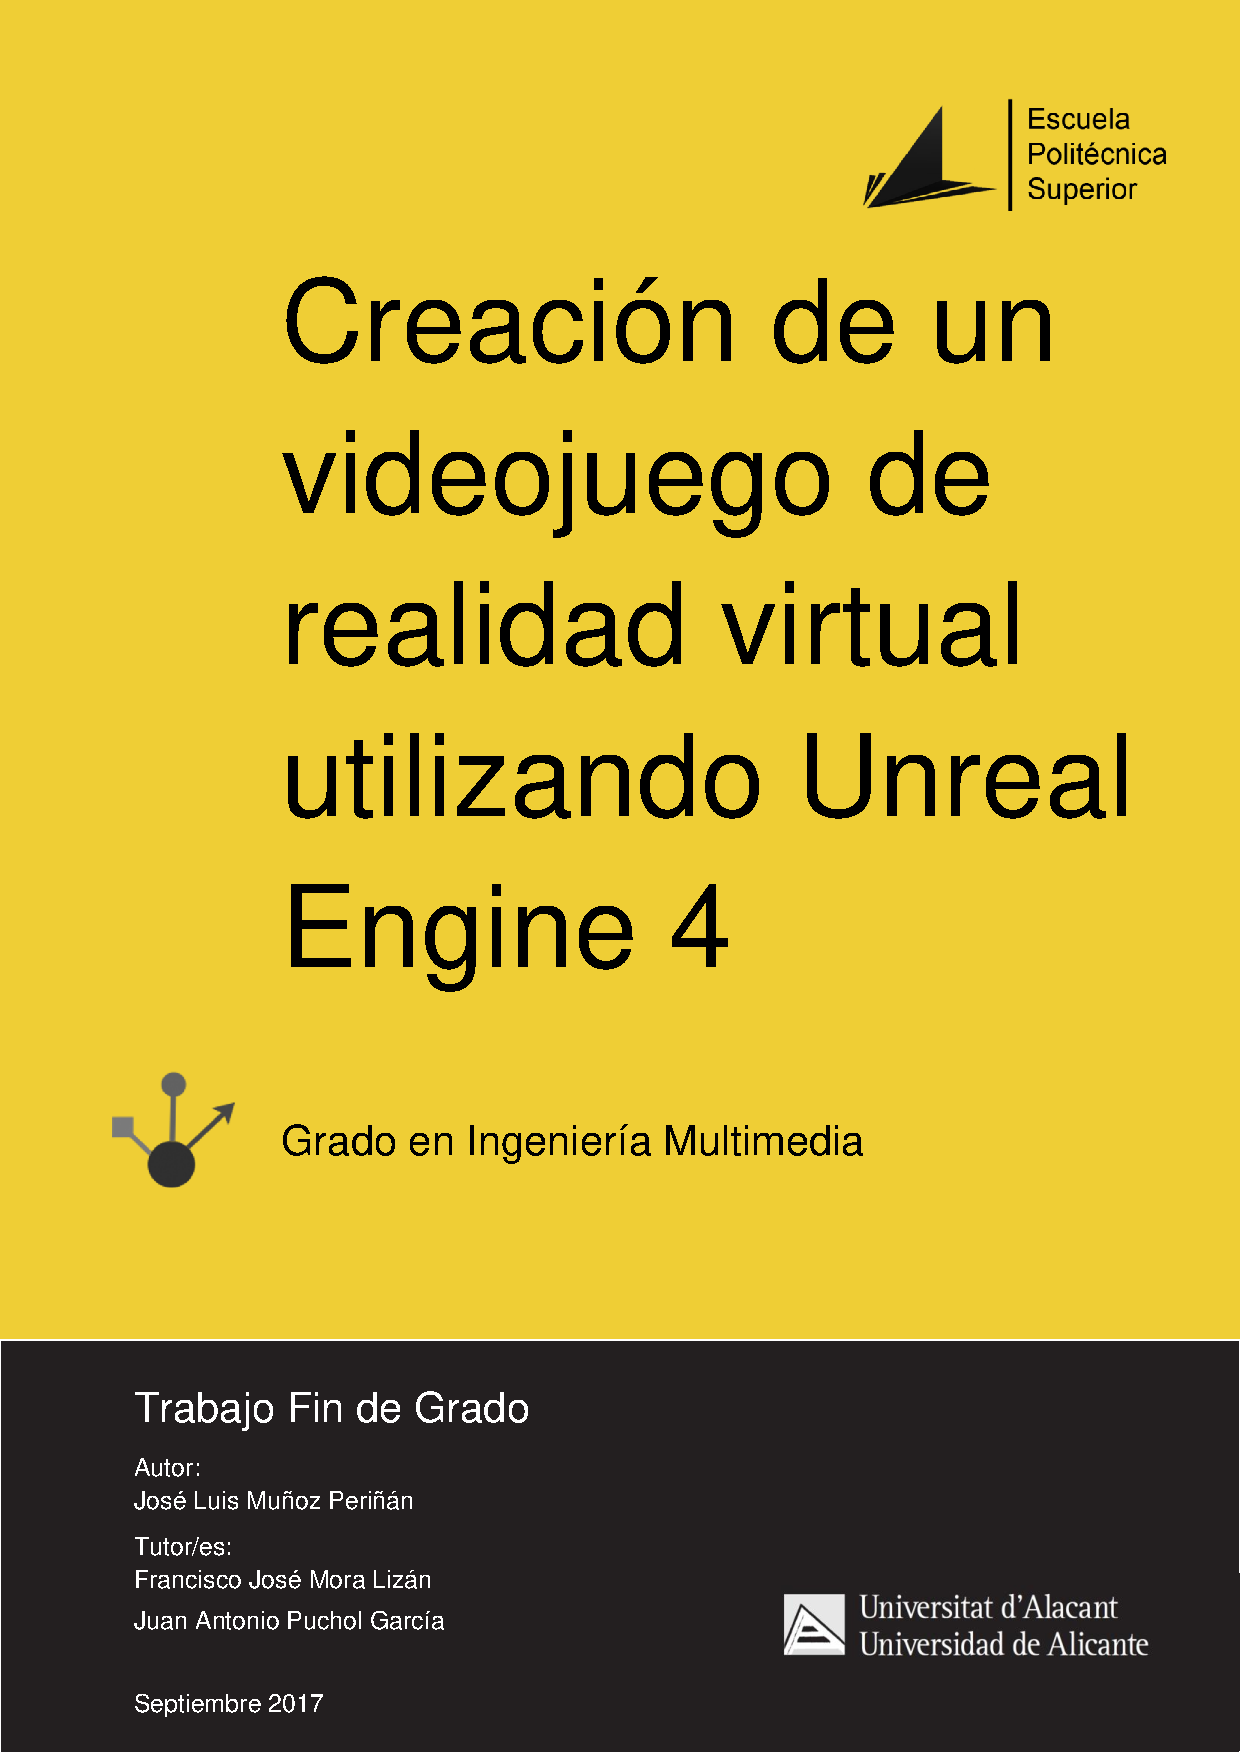
\includepdf[pages={1},pagecommand={},fitpaper=true,trim=0 0 0 0, 
offset=0 0,turn=true,noautoscale=true]{portada/portada.pdf}

\end{titlepage}
\pagecolor{white} %la portada en color
\begin{titlepage}
 
 
\setlength{\centeroffset}{-0.5\oddsidemargin}
\addtolength{\centeroffset}{0.5\evensidemargin}
\thispagestyle{empty}

\noindent\hspace*{\centeroffset}\begin{minipage}{\textwidth}

\centering


% Title

%{\Huge\bfseries Título del proyecto\\ }
{\Huge\bfseries \myTitle}

\noindent\rule[-1ex]{\textwidth}{3pt}\\[3.5ex]
%{\large\bfseries \mySubtitle\\[4cm]}
\end{minipage}

\vspace{2.5cm}
\noindent\hspace*{\centeroffset}\begin{minipage}{\textwidth}
\centering

\textbf{Autor}\\ {\myName}\\[2.5ex]
\textbf{Directores}\\
{\normalsize \myProf\\
\small\textit \depTutorOne\\
\normalsize \myOtherProf\\
\small\textit \depTutorTwo\\[2cm]}

\includegraphics[scale=0.25]{\logoGrado}


\textsc{\myDegree}\\

\centering
\begin{minipage}[l]{7cm}
\includegraphics[width=5cm]{\logoFacultad}
\end{minipage}
\begin{minipage}[r]{7cm}
\includegraphics[width=5cm]{\logoUniversidad}
\end{minipage}


%\textsc{\myFaculty}\\

%\large\bfseries \textsc{\myUni}\\
ALICANTE, \myTime

\end{minipage}
%\addtolength{\textwidth}{\centeroffset}
\vspace{\stretch{2}}

\end{titlepage}


 %la portada en b/n
\chapter*{Preámbulo}
\thispagestyle{empty}
Poner aquí un texto breve que debe incluir entre otras:
\begin{quote}
``las razones que han llevado a la realización del estudio, el tema, la finalidad y el alcance y también los agradecimientos por las ayudas, por ejemplo apoyo económico (becas y subvenciones) y las consultas y discusiones con los tutores y colegas de trabajo. \cite{UNE50136:97}''
\end{quote}

\cleardoublepage %salta a nueva página impar
% Aquí va la dedicatoria si la hubiese. Si no, comentar la(s) linea(s) siguientes
\chapter*{}
\setlength{\leftmargin}{0.5\textwidth}
\setlength{\parsep}{0cm}
\addtolength{\topsep}{0.5cm}
\begin{flushright}
\small\em{
A mi esposa Marganit, y a mis hijos Ella Rose y Daniel Adams,\\
sin los cuales habría podido acabar este libro dos años antes \footnote{Dedicatoria de Joseph J. Roman en ``An Introduction to Algebraic Topology''}
}
\end{flushright}


\cleardoublepage %salta a nueva página impar
% Aquí va la cita célebre si la hubiese. Si no, comentar la(s) linea(s) siguientes
\chapter*{}
\setlength{\leftmargin}{0.5\textwidth}
\setlength{\parsep}{0cm}
\addtolength{\topsep}{0.5cm}
\begin{flushright}
\small\em{
Si consigo ver más lejos\\
es porque he conseguido auparme\\ 
a hombros de gigantes
}
\end{flushright}
\begin{flushright}
\small{
Isaac Newton.
}
\end{flushright}
\cleardoublepage %salta a nueva página impar
 %editar este texto (capitulos/preliminares.tex) para cambiar preámbulo, agradecimientos y dedicatorias
\tableofcontents
\listoffigures
\listoftables
\lstlistoflistings

\mainmatter %entre frontmatter y mainmatter, la numeración es en romanos.

%a continuación se propone un esquema de trabajo que puede ser alterado justificadamente.
\acresetall{}  % resetea los acrónimos por si han sido usados en el índice o en los preliminares.
\chapter{Introducción}

Hoy en día la industria del videojuego es uno de los mercados más potentes de nuestra economía. Con el paso de los años este sector se ha ido extendiendo y normalizando hasta llegar al punto en el que se ha convertido en algo que aparece con total normalidad en nuestra vida cotidiana.

Hay todo tipo de juegos, desde sencillos juegos de móviles a grandes producciones que no tienen nada que enviar a las grandes películas con presupuestos millonarios de Hollywood, no es de extrañar que mucha gente considere el videojuego como \textit{el décimo arte.}

\section{Estructura de un \ac{TFG}}

En caso de que el \ac{TFG}/\acs{TFM} tenga como finalidad la elaboración de un proyecto o un 
informe científico o técnico, deberá ajustarse a lo dispuesto en las normas UNE 
157001:2002 y UNE 50135:1996 respectivamente.

Si el \ac{TFG}/\ac{TFM} tiene por finalidad la elaboración de un trabajo monográfico, el 
documento presentado deberá constar de las siguientes partes, teniendo como base la 
norma UNE 50136:1997.

\begin{description}
\item[Preámbulo:] se describirán brevemente la motivación que ha originado la realización del \ac{TFG}/\acs{TFM}, así como de una breve descripción de los objetivos generales que se quieren alcanzar con el trabajo presentado.
\item[Agradecimientos:] se podrá añadir las hojas necesarias para realizar los agradecimientos, a veces obligatorios, a las entidades y organismos colaboradores.
\item[Dedicatoria:] se podrá añadir una única hoja con dedicatorias, su alineación será derecha y centradas de forma distribuida en la página.
\item[Citas:] (frases célebres) se podrá añadir una única hoja con citas, su alineación será derecha y centradas de forma distribuida en la página.
\item[Índices:] cada índice debe comenzar en una nueva página, se incluirán los índices que se estimen necesarios (conforme UNE 50111:1989), en este orden:
\begin{description}
\item[Índice de contenidos:] (obligatorio siempre) se incluirá un índice de las secciones de las que se componga el documento, la numeración de las 
divisiones y subdivisiones utilizarán cifras arábigas (según UNE 50132:1994) y harán mención a la página del documento donde se ubiquen.
\item[Índice de figuras:] si el documento incluye figuras se podrá incluir también un índice con su relación, indicando la página donde se ubiquen.
\item[Índice de tablas:] en caso de existir en el texto, ídem que el anterior.
\item[Índice de abreviaturas, siglas, símbolos, etc.:] en caso de ser necesarios se podrá incluir cada uno de ellos.
\end{description}
\item[Cuerpo del documento:] en el contenido del documento se da flexibilidad para su organización y se puede estructurar en las secciones que se considere. En todo caso obligatoriamente se deberá, al menos, incluir los siguientes contenidos:
\begin{description}
\item[Introducción:] donde se hará énfasis a la importancia de la temática, su vigencia y actualidad; se planteará el problema a investigar, así como el propósito o finalidad de la investigación.
\item[Marco teórico o Estado del arte:] se hará mención a los elementos conceptuales que sirven de base para la investigación, estudios previos relacionados con el problema planteado, etc.
\item[Objetivos:] se establecerá el objetivo general y los específicos.
\item[Metodología:] se indicará el tipo o tipos de investigación, las técnicas y los procedimientos que serán utilizados para llevarla a cabo; se identificará la población y el tamaño de la muestra así como las técnicas e instrumentos de recolección de datos.
\item[Resultados:] incluirá los resultados de la investigación o trabajo, así como el análisis y la discusión de los mismos.
\end{description}
\item[Conclusiones:] obligatoriamente se incluirá una sección de conclusiones donde se realizará un resumen de los objetivos conseguidos así como de los resultados obtenidos si proceden.
\item[Bibliografía y referencias:] se incluirá también la relación de obras y materiales consultados y empleados en la elaboración de la memoria del \ac{TFG}/\ac{TFM}. La bibliografía y las referencias serán indexadas en orden alfabético (sistema nombre y fecha) o se numerará correlativamente según aparezca (sistema numérico). Se empleará la familia 1 como tipo de letra. Podrá utilizarse cualquier sistema bibliográfico normalizado predominante en la rama de conocimiento, estableciéndose como prioritarios el sistema ISO 690, sistema \ac{APA}  o Harvard (no necesariamente en ese orden de preferencia). En esta plantilla Latex se propone usar el estilo \ac{APA} indicándolo en la línea correspondiente como 
\begin{verbatim}
\bibliographystyle{apalike}
\end{verbatim}


\item[Anexos:] se podrá incluir los anexos que se consideren oportunos.

\end{description}




\chapter{Marco Teórico o  Estado del arte}
\label{marcoteorico}

En este apartado hablaré del concepto de videojuego y lo que define a un juego del género de terror. Para ello buscaré ejemplos en la industria, desde pequeños juegos realizados por estudios independientes (\textit{indies}) hasta grandes producciones de videojuegos realizadas por las principales empresas del sector.

\section{¿Que es un videojuego?}

Basta con buscar un poco por Internet para encontrar la siguiente definición de videojuego:
\\

\textit{Un videojuego es un juego electrónico en el que una o más personas interactúan, por medio de un controlador, con un dispositivo que muestra imágenes de vídeo. Este dispositivo electrónico puede ser una computadora, una máquina arcade, una videoconsola o un dispositivo portátil.}\footnote{Definición encontrada en la página de la Wikipedia: \url{https://es.wikipedia.org/wiki/Videojuego}.}
\\

Cada medio o autor usa sus propias palabras para definir lo que es un videojuego, sin embargo esta podría ser considerada la definición básica del término.
\\

A pesar de que ya habían juegos antes que ellos, los primeros videojuegos que triunfaron entre el gran público fueron juegos como \textit{Computer Space} (1971) o \textit{Pong} (1972). Este último tuvo especial éxito, siendo considerado como el juego más importante de la primera generación de videojuegos.
\\

El \textit{Pong} es un juego muy simple: es un juego de deportes de dos dimensiones que consiste en mover verticalmente una paleta para golpear una pelota y enviarla al campo del contrario. Cada vez que un jugador falla en golpear la bola el contrincante anota un punto, gana el jugador con más puntos.
\\


\begin{figure}
	\begin{center}
		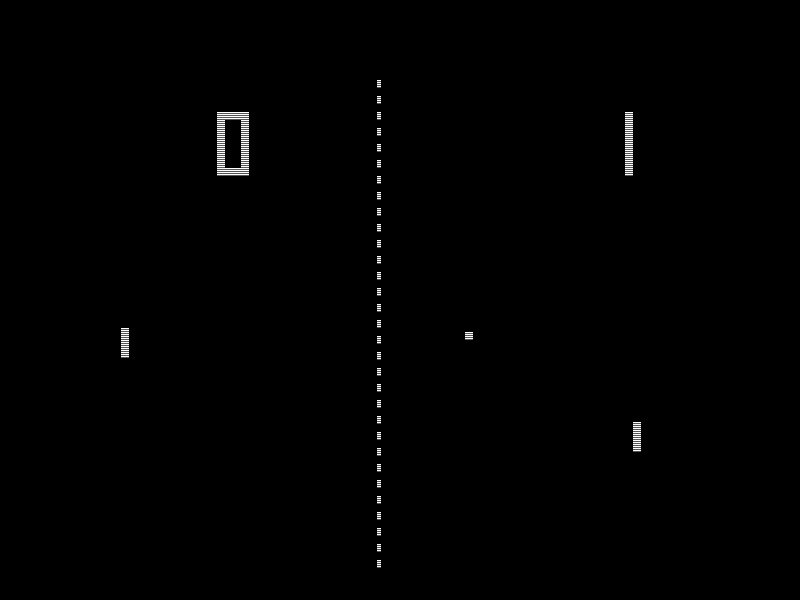
\includegraphics[scale=0.3]{imagenes/Pong.png}
		\caption{\textit{Pong}, el primer videojuego con un gran éxito comercial.}
		\label{spacewar}
	\end{center}
\end{figure}

El \textit{Pong} es un claro ejemplo de que con el paso de los años los videojuegos han evolucionado en todos los sentidos y se han hecho más accesibles entre el gran público. Al tener más éxito la industria ha concebido juegos cada vez más complejos.
\\

Hoy en día existen juegos de multitud de géneros como resultado de esa larga evolución, lejos queda ya esa época en la que el género Arcade eclipsaba todo el panorama de videojuegos, ahora existen un gran número de juegos capaces de contarte multitud de historias y con una amplia variedad de géneros y mecánicas.
\\


\section{Videojuego de terror}

El videojuego de terror ha evolucionado también mucho en los últimos años, los que podrían ser considerados los padres del género (como Resident Evil o Silent Hill) ya no tienen tanta relevancia en el espectro actual, aunque siguen siendo muy influyentes. 
\\

Para la realización de este videojuego se han observado y analizado un gran número de juegos de miedo, la mayoría son juegos recientes que aprovechan las últimas tendencias y cuyas mecánicas se pueden adaptar a la realidad virtual:

\begin{itemize}
	\item Outlast
	\item P.T.
	\item Alien: Isolation
	\item The Evil Within
	\item Resident Evil VII
\end{itemize}

\subsection{Outlast}

\begin{figure}
	\begin{center}
		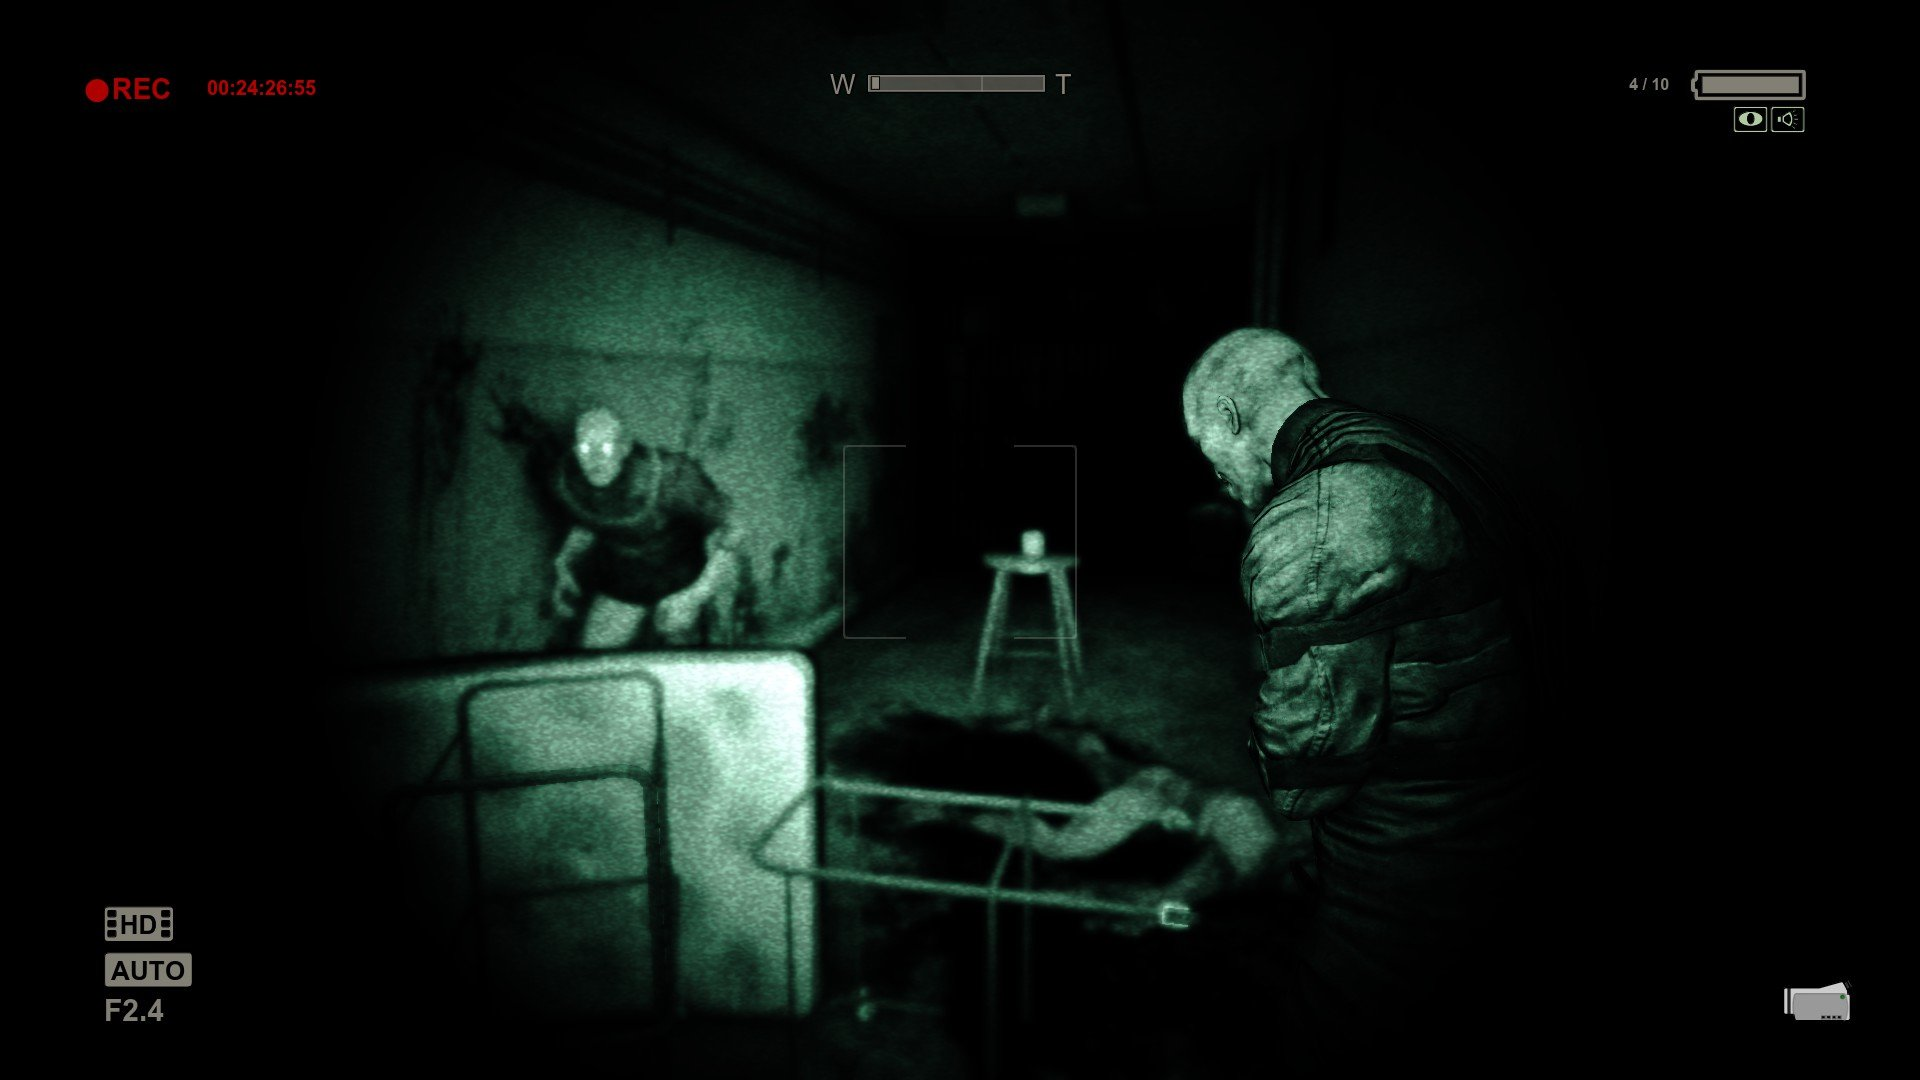
\includegraphics[scale=0.2]{imagenes/Outlast.jpg}
		\caption{Imagen \textit{in-game} de \textit{Outlast}.}
		\label{outlast}
	\end{center}
\end{figure}

Outlast es un videojuego de terror en primera persona desarrollado por el estudio canadiense \textit{Red Barrels Games} en 2013. En este juego eres un periodista encerrado en un psiquiátrico sobrenatural. 
\\

Este juego tiene varias mecánicas interesantes, en primer lugar, todo el juego gira en función a una cámara de vídeo que llevamos encima, ya que tiene visión nocturna y nos permite ver en los lugares más oscuros, por lo que es importante rastrear el escenario en busca de baterías para la cámara.
\\

Otro punto interesante de este juego es que no hay ninguna manera de atacar a los enemigos, por lo que siempre que te encuentras una amenaza tienes que huir. Esta mecánica, aunque puede llegar a ser frustrante, aumenta la sensación de infedensión, por lo que el miedo que se experimenta jugando es mucho mayor, ya que te sientes mucho más expuesto. Esta es una mecánica que me ha convencido y que se lleva practicando en algunos juegos desde hace un tiempo, por lo que he decidido implementarla en \textbf{\nombreJuego}.
\\

\subsection{P.T.}

\begin{figure}
	\begin{center}
		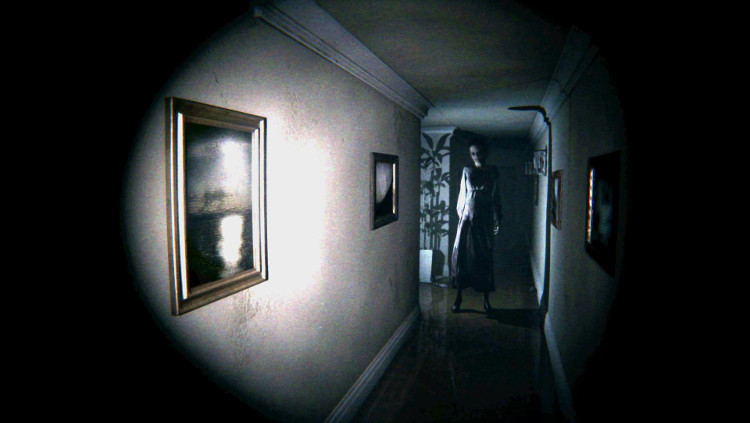
\includegraphics[scale=0.50]{imagenes/PT.jpg}
		\caption{Imagen \textit{in-game} de \textit{P.T.}}
		\label{PT}
	\end{center}
\end{figure}

Este juego me parece especialmente interesante, ya que no es un videojuego como tal, sino un \textit{teaser} de lo que iba a ser un nuevo \textit{Silent Hill} que nunca llego a ver la luz.
\\

Este juego fue desarrollado por \textbf{Hideo Kojima}, director de los famosos \textit{Metal Gear}, en colaboración con Guillermo Del Toro, director de películas como \textit{HellBoy} o \textit{Pacific Rim}. El juego estuvo disponible de manera gratuita durante un tiempo en 2014 y fue un éxito por parte del público y la crítica.
\\

Es un juego en tercera persona que transcurre en una pequeña casa donde ocurren fenómenos paranormales.Para superar el juego el jugador debe avanzar por las estancias de la casa superando algunos puzles. Este juego tampoco tiene una mecánica que implique usar la violencia, volviendo a esa sensación de indefensión que he mencionado anteriormente. Es un juego muy corto y que provoca un miedo principalmente atmosférico, causando una tensión constante en el jugador.
\\

Quiero destacar este juego porque me ha parecido especialmente interesante, sobre todo por la atmósfera y el arte, por lo que es uno de los principales referentes de \textbf{\nombreJuego}.
\\

\subsection{Alien: Isolation}

\begin{figure}
	\begin{center}
		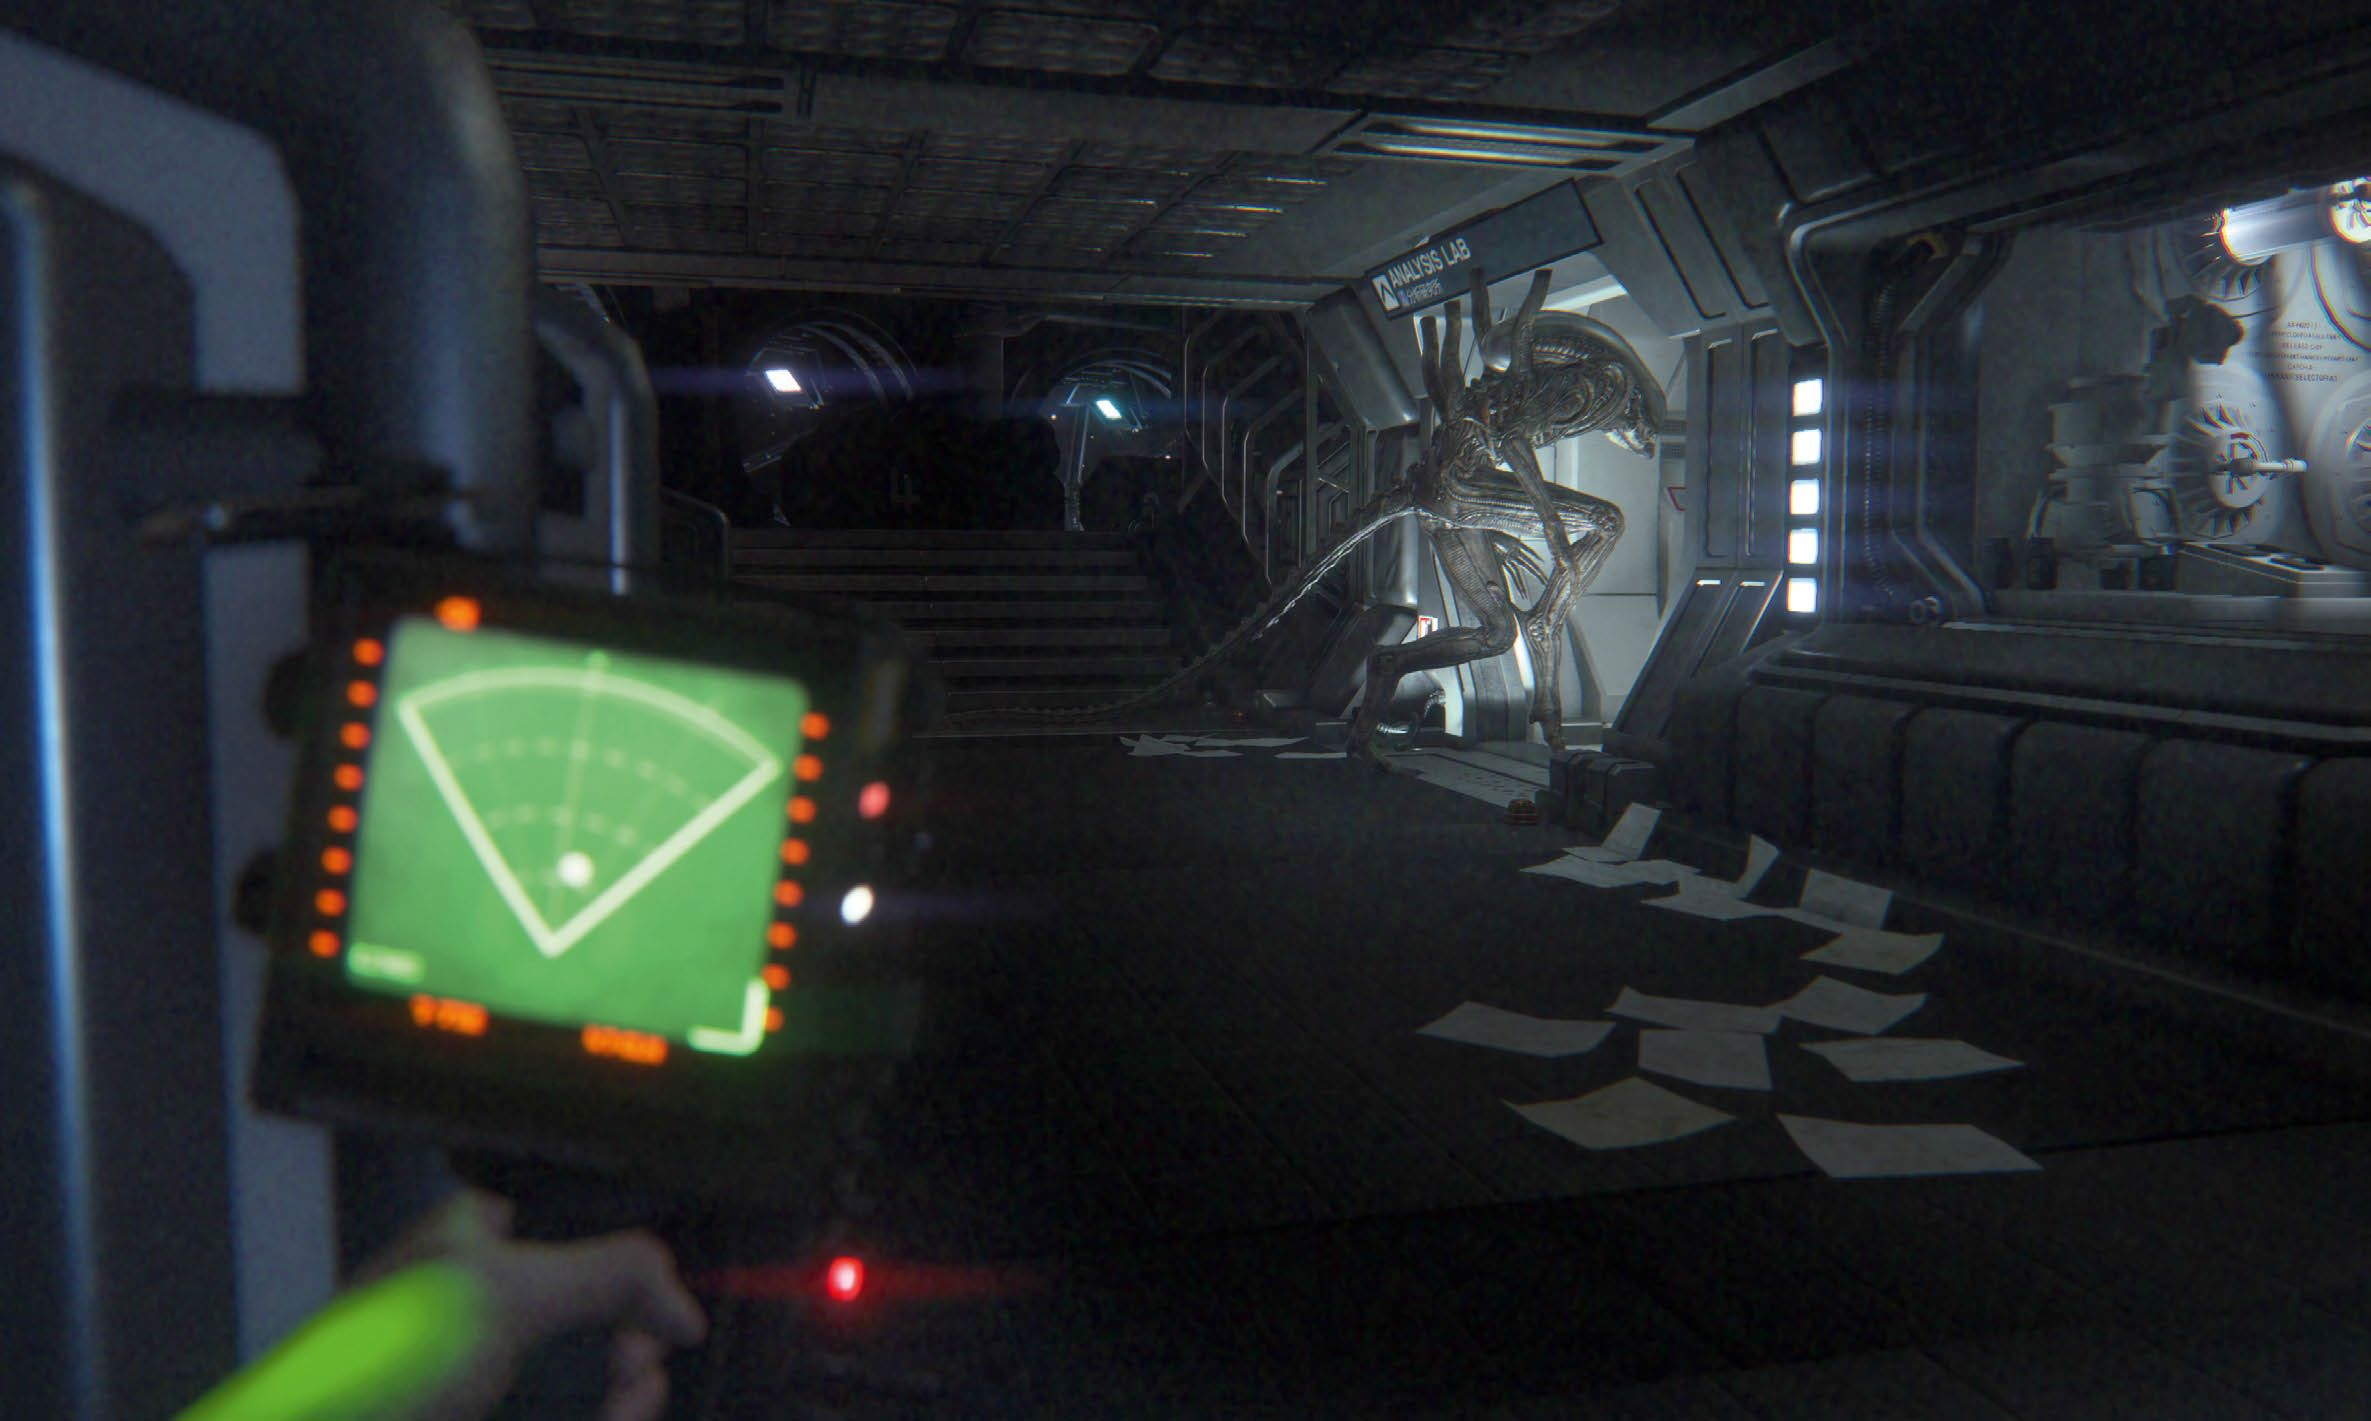
\includegraphics[scale=0.16]{imagenes/alien.jpg}
		\caption{Imagen \textit{in-game} de \textit{Alien: Isolation}.}
		\label{alien}
	\end{center}
\end{figure}

Este juego desarrollado por \textit{The Creative Assembly} en 2014 es un juego de terror y sigilo en primera persona basado en la franquicia de películas \textit{Alien}.
\\

Este juego transcurre en una nave destrozada en la que está libre el \textit{xenomorfo}, la principal mecánica del videojuego consiste en esconderse y escapar del alien. 
\\

Aunque en este juego si que dispones de herramientas para defenderte, a la hora de la verdad resultan inútiles contra el enemigo y tu mejor baza que tienes es escapar; otra vez más se repite ese sentimiento de desprotección, lo que aumenta considerablemente el miedo y la tensión al jugar.

\subsection{The Evil Within}

\begin{figure}
	\begin{center}
		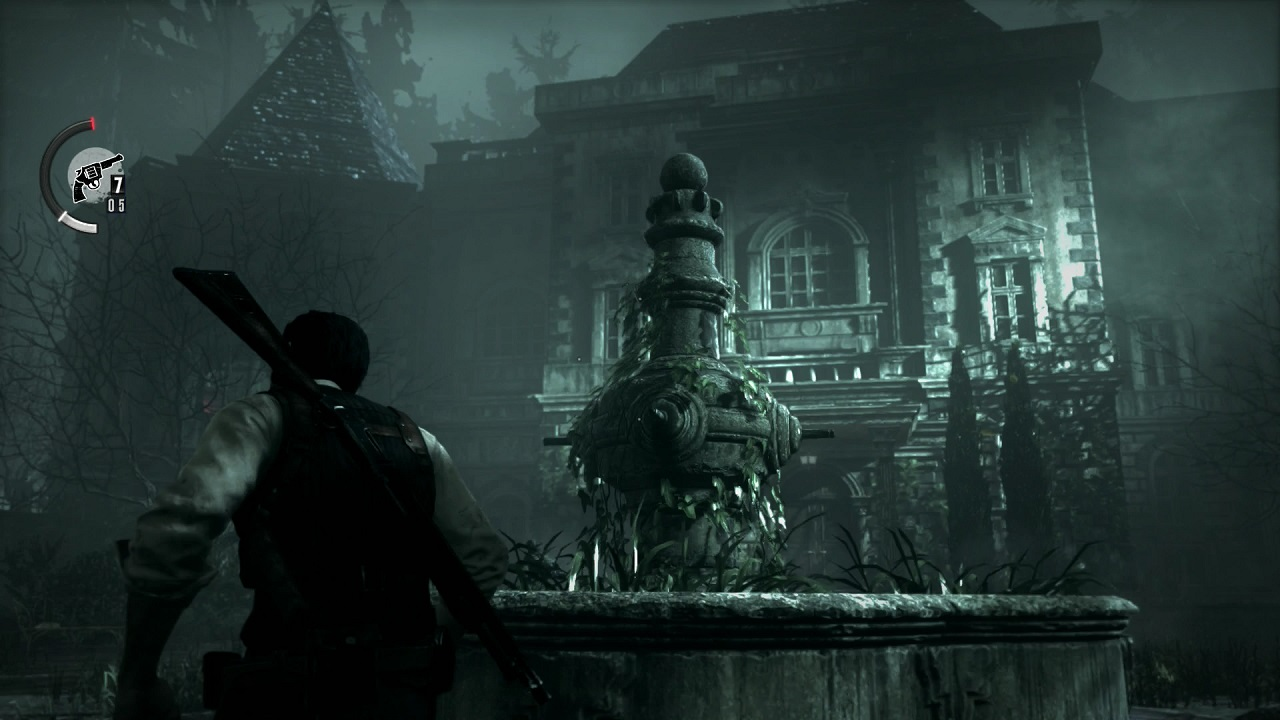
\includegraphics[scale=0.52]{imagenes/EvilWithin.jpg}
		\caption{Imagen \textit{in-game} de \textit{The Evil Within}.}
		\label{EvilWithin}
	\end{center}
\end{figure}

\textit{The Evil Within} es un juego bastante diferente a los anteriores, ya que incluye muchas mecánicas y partes de acción. No obstante es un juego destacable ya que ha tenido cierto éxito desde su salida en 2014.
\\

Este juego fue desarrollado por Shinji Mikami, creador de la saga \textit{Resident Evil}, unos de los padres del género. Es un juego de terror y acción en tercera persona, trata de un agente de policía que se tiene que enfrentar a ciertos fenómenos paranormales. En este juego te enfrentas directamente a muchos enemigos, usando armas de fuego o de cuerpo a cuerpo, además tienes que resolver un buen número de puzles para completar el juego.
\\

Este juego destaca entre otras cosas por lo grotesco de los enemigos y los escenarios, cuenta con un apartado artístico muy desagradable, proporcionando una sensación de incomodidad constante al jugador. Esto último resulta muy interesante, pero he decidido no incluir nada parecido en \nombreJuego, ya que las características de los juegos que he hablado anteriormente me han convencido más. No obstante, me ha parecido un juego con algunas propuestas interesantes e ideas que se pueden adaptar a \textbf{\nombreJuego}.

\subsection{Resident Evil VII}

\begin{figure}
	\begin{center}
		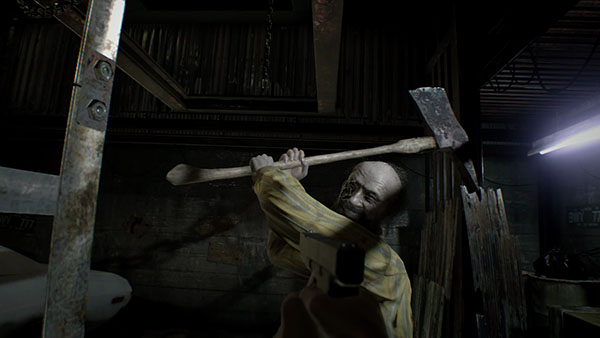
\includegraphics[scale=0.65]{imagenes/REVII.jpg}
		\caption{Imagen \textit{in-game} de \textit{Resident Evil VII}.}
		\label{ResidentEvil}
	\end{center}
\end{figure}

Para concluir este apartado, quiero mencionar el que es el principal referente para \textbf{\nombreJuego} junto a P.T. El Resident Evil VII es un juego que salió el pasado año y que supone la vuelta de la principal franquicia de juegos de terror.
\\

Este es un juego muy interesante, ya que toma las principales mecánicas de los juegos de terror en los últimos años y se adapta a ellas manteniendo la esencia de la franquicia.
\\

Es un juego en primera persona con mecánicas de acción con disparos que se desarrolla en una mansión. Para avanzar por la casa tienes que ir resolviendo ciertos puzles que desbloquean nuevas estancias y que hacen que avance la trama del juego. En este sentido el juego es muy semejante a P.T., ya que ambos juegos desarrollan la acción en un recinto cerrado donde la ambientación y la atmósfera de la casa ponen en una tensión constante al jugador.
\\
Quiero destacar además que este juego es totalmente compatible con dispositivos de realidad virtual, estando ya disponible para las gafas \textit{Playstation VR} y en un futuro para otros dispositivos.
\\








\begin{comment}
El contenido de este capítulo es una especie de muestrario de cosas que puedes hacer con \LaTeX.  Por ejemplo, incluir una cita bibliográfica   \cite{BOE_IM_UA} dentro del texto. En esta página de demostración también puedes encontrar información útil acerca de cómo escribir con  \LaTeX.\footnote{En http://metodos.fam.cie.uva.es/~latex/apuntes/apuntes.html hay unos buenos apuntes al respecto.}
\section{Listas}
Hacer una lista es simple en \LaTeX. Para ello has de crear un entorno (así se llama) itemize con
\begin{verbatim}
\begin{itemize}
...
\end{itemize}
\end{verbatim}
Y dentro de esa estructura, añadir cada elemento de la lista precedido de 
\begin{verbatim}
\item primer item de lista
\item segundo item de lista
...
\item ultimo item de lista
\end{verbatim}

Es importante que revises este texto tal como aparece en la plantilla y relaciones el aspecto que tiene el PDF final con cómo está escrito el documento \LaTeX.

Aquí va una lista:
\begin{itemize}
    \item Ingeniería Informática.
    \item Ingeniería Sonido e Imagen en Telecomunicación.
    \item Ingeniería Multimedia.
    \begin{itemize}
         \item Mención: Creación y ocio digital.
         \item Mención: Gestión de Contenidos.
    \end{itemize}
\end{itemize}


\section{Tablas}
Ahora veremos otra estructura más: las tablas.

\subsection{Inserción de tablas}

Aquí va una tabla\footnote{En http://www.tablesgenerator.com/ se puede encontrar un generador On-Line de tablas para \LaTeX} para que se vea cómo insertar una tabla simple dentro del documento.

\begin{table}[h]
\begin{center}
\begin{tabular}{lllll}
&columna A&columna B&columna C\\
\hline
fila 1&fila 1, columna A & fila 1, columna B & fila 1, columna C\\
fila 2&fila 2, columna A & fila 2, columna B & fila 2, columna C\\
fila 3&fila 3, columna A & fila 3, columna B & fila 3, columna C\\ \hline
\end{tabular}
\end{center}
\caption{Ejemplo de tabla.}
\label{tabladeejemplo}
\end{table}

\LaTeX usa un sistema de parámetros para ``decorar'' las tablas. Puedes consultar estos parámetros en la tabla \ref{tabla_parametros} de la página \pageref{tabla_parametros}. La tabla se ubicará donde, a juicio de \LaTeX, menos moleste por lo que puede no aparecer necesariamente donde se ha insertado en el texto original. 

\begin{table}
\begin{center}
\begin{tabular}{|c|p{0.8\textwidth}|}
\hline
Parámetro & \multicolumn{1}{c|}{Significado} \\ \hline
\texttt{h} & Situa el elemento flotante \emph{preferentemente}
(es decir, si es posible) en la situación exacta donde se incluye este \\
\texttt{t} & Situa el elemento en la parte de arriba de la página \\
\texttt{b} & Situa el elemento en la parte de abajo de la página \\
\texttt{p} & Situa el elemento en una página aparte dedicada sólo a
elementos flotantes; en el caso del formato \texttt{article},
ésta se situa al final del documento, mientras que para al book es
colocada al final de cada capítulo \\ \hline
\end{tabular}
\end{center}
\caption{Parámetros optativos de los entornos flotantes}
\label{tabla_parametros}
\end{table}



\section{Inserción de figuras}

Las figuras son un caso un poco especial ya que \LaTeX busca el mejor lugar para ponerlas, no siendo necesariamente el ligar donde está la referencia. Por ello es importante añadirle un ``caption'' y un ``label'' para poder hacer referencia a ellas en el párrafo correspondiente. Nosotros ponemos la referencia a la figura \ref{logo_im} que está en la página \pageref{logo_im}. justo aquí debajo, pero \LaTeX puede que la ubique en otro lugar.

\begin{figure}
\begin{center}

\includegraphics[scale=0.25]{imagenes/logoim.jpg}
\caption{Logo de Ingeniería  Multimedia.}
\label{logo_im}
\end{center}
\end{figure}

\begin{figure}
\begin{center}

\includegraphics[scale=0.25]{imagenes/logoeps.jpg}
\caption{Logo de la EPS.}
\label{logo_eps}
\end{center}
\end{figure}

\section{Inserción de código}
A veces tendrás que insertar algún pedazo de código fuente para explicar algo relacionado con él. No sustituyas explicaciones con enormes listados de código. Si pones algo de código en tu TFG que sea para demostrar algo o explicar alguna solución.

\LaTeX te ayuda a escribir código de manera que su presentación tenga las marcas y tabulaciones propias de este tipo de texto. Para ello, debes poner el código que escribas DENTRO de un entorno  que se llama ``listings''.  La plantilla ya tiene una serie de instrucciones para incluir el paquete ``listings'' y añadirle algunos modificadores por lo que no tienes que incluirlo tú. Simplemente, mete tu código en el entorno ``lstlisting'' y ya está. Puedes indicar el lenguaje en el que está escrito el código y así \LaTeX lo mostrará mejor. Veamos un ejemplo en la figura \ref{C_code}:

Si pones 
\begin{verbatim}
\begin{lstlisting}[style=C, caption={ejemplo código C},label=C_code]
#include <stdio.h>
int main(int argc, char* argv[]) {
  puts("Hola mundo!");
}
\end{lstlisting}
\end{verbatim}

El resultado será:
\begin{lstlisting}[style=C, caption={ejemplo código C},label=C_code]
#include <stdio.h>
int main(int argc, char* argv[]) {
  puts("Hola mundo!");
}
\end{lstlisting}

Por supuesto, puedes mejorar esta presentación utilizando mas modificadores. Esta información y mucha más puede ser encontrada en \cite{listing_packagge} y en \cite{heinz1listings}.

Otro ejemplo, ahora para mostrar código PHP, sería escribir en tu fichero \LaTeX lo siguiente:
\begin{verbatim}
 \begin{lstlisting}[style=PHP, caption={ejemplo código PHP},label=PHP_code]
 /* 
Ejemplo de código en PHP para escribir tu primer programa en este lenguaje
Copia este código en tu ordenador y ejecútalo
*/
<html>
  <head>
    <title>Prueba de PHP</title>
  </head>
  <body>
    <?php echo '<p>Hola Mundo</p>'; ?> //esto lo escribe TODO el mundo
  </body>
</html>
 \end{lstlisting}
\end{verbatim}
 
 y el resultado es: (ver listado \ref{PHP_code})
 
 \begin{lstlisting}[style=PHP, caption={ejemplo código PHP},label=PHP_code]
/* 
Ejemplo de código en PHP para escribir tu primer programa en este lenguaje. Copia este código en tu ordenador y ejecútalo
*/
 <html>
  <head>
    <title>Prueba de PHP</title>
  </head>
  <body>
    <?php echo '<p>Hola Mundo</p>'; ?> //esto lo escribe TODO el mundo
  </body>
</html>
 \end{lstlisting}
 
 Observa cómo \LaTeX ha puesto los comentarios en gris y ajustado el código para que se muestre más claro.
 
 Si quieres añadir código en otros lenguajes, cambia el comando que dice 
 
 \begin{center}
 ``style=nombredellenguaje''
 
  por 
 
 ``languaje=nombredelnuevolenguaje''.
 \end{center}
 
 \section{Acrónimos}
 Por último vamos a ver cómo se ponen los acrónimos.
 
 La norma dice que la primera vez que aparece un acrónimo debe ponerse su fórmula completa es decir, lo que significa, al lado del acrónimo. Después de ello, podemos usar ya sólo el acrónimo salvo cuando consideremos que debemos volver a usar la fórmula completa por alguna razón de legibilidad.
 
 ¿Cómo llevar la cuenta de cuándo es la primera vez que ponemos el acrónimo? si hacemos cambios en el doc es fácil que perdamos esa información así que lo mejor es que sea el propio \LaTeX  el que lleve esa cuenta. Para ello tenemos que hacer dos cosas:
 \begin{description}
 \item[Primero:] creamos la entrada del acrónimo en el fichero acronimos.tex. Revisad los comentarios de su cabecera para saber cómo crear esa entrada. Básicamente lo que hacemos allí es poner la ``fórmula corta'' y la ``fórmula larga'' del acrónimo es decir, el propio acrónimo y su significado
 \item[Segundo:] escribimos en el texto el acrónimo SIEMPRE diciendo que es un acrónimo y el tipo de fórmula que queremos usar. Por ejemplo, si siempre que queremos hacer referencia al IEEE escribimos \begin{verbatim}\ac{IEEE}\end{verbatim}  se consigue que la primera vez que aparezca el acrónimo ponga las fórmulas larga y la corta y en las siguientes ocasiones sólo aparecerá la corta.
 \end{description}
 
 Aquí va un ejemplo:
 
 Si escribimos:
 
 \begin{verbatim}
 El \ac{IEEE} es una institución muy importante en el mundo de la
 ingeniería.  El \ac{IEEE} lleva marcando normas y protocolos desde
 hace mucho tiempo.  Pero el \acf{IEEE} no está solo en esta tarea. 
 Además del \ac{IEEE} hay muchas otras instituciones para ello.
 \end{verbatim}
 
 Obtendremos: 
 
El \ac{IEEE} es una institución muy importante en el mundo de la ingeniería. El \ac{IEEE} lleva marcando normas y protocolos desde hace mucho tiempo. Pero el \acl{IEEE} no está solo en esta tarea. Además del \ac{IEEE} hay muchas otras instituciones para ello.

\end{comment}
 
\chapter{Introducción}

Hoy en día la industria del videojuego es uno de los mercados más potentes de nuestra economía. Con el paso de los años este sector se ha ido extendiendo y normalizando hasta llegar al punto en el que se ha convertido en algo que aparece con total normalidad en nuestra vida cotidiana.

Hay todo tipo de juegos, desde sencillos juegos de móviles a grandes producciones que no tienen nada que enviar a las grandes películas con presupuestos millonarios de Hollywood, no es de extrañar que mucha gente considere el videojuego como \textit{el décimo arte.}

\section{Estructura de un \ac{TFG}}

En caso de que el \ac{TFG}/\acs{TFM} tenga como finalidad la elaboración de un proyecto o un 
informe científico o técnico, deberá ajustarse a lo dispuesto en las normas UNE 
157001:2002 y UNE 50135:1996 respectivamente.

Si el \ac{TFG}/\ac{TFM} tiene por finalidad la elaboración de un trabajo monográfico, el 
documento presentado deberá constar de las siguientes partes, teniendo como base la 
norma UNE 50136:1997.

\begin{description}
\item[Preámbulo:] se describirán brevemente la motivación que ha originado la realización del \ac{TFG}/\acs{TFM}, así como de una breve descripción de los objetivos generales que se quieren alcanzar con el trabajo presentado.
\item[Agradecimientos:] se podrá añadir las hojas necesarias para realizar los agradecimientos, a veces obligatorios, a las entidades y organismos colaboradores.
\item[Dedicatoria:] se podrá añadir una única hoja con dedicatorias, su alineación será derecha y centradas de forma distribuida en la página.
\item[Citas:] (frases célebres) se podrá añadir una única hoja con citas, su alineación será derecha y centradas de forma distribuida en la página.
\item[Índices:] cada índice debe comenzar en una nueva página, se incluirán los índices que se estimen necesarios (conforme UNE 50111:1989), en este orden:
\begin{description}
\item[Índice de contenidos:] (obligatorio siempre) se incluirá un índice de las secciones de las que se componga el documento, la numeración de las 
divisiones y subdivisiones utilizarán cifras arábigas (según UNE 50132:1994) y harán mención a la página del documento donde se ubiquen.
\item[Índice de figuras:] si el documento incluye figuras se podrá incluir también un índice con su relación, indicando la página donde se ubiquen.
\item[Índice de tablas:] en caso de existir en el texto, ídem que el anterior.
\item[Índice de abreviaturas, siglas, símbolos, etc.:] en caso de ser necesarios se podrá incluir cada uno de ellos.
\end{description}
\item[Cuerpo del documento:] en el contenido del documento se da flexibilidad para su organización y se puede estructurar en las secciones que se considere. En todo caso obligatoriamente se deberá, al menos, incluir los siguientes contenidos:
\begin{description}
\item[Introducción:] donde se hará énfasis a la importancia de la temática, su vigencia y actualidad; se planteará el problema a investigar, así como el propósito o finalidad de la investigación.
\item[Marco teórico o Estado del arte:] se hará mención a los elementos conceptuales que sirven de base para la investigación, estudios previos relacionados con el problema planteado, etc.
\item[Objetivos:] se establecerá el objetivo general y los específicos.
\item[Metodología:] se indicará el tipo o tipos de investigación, las técnicas y los procedimientos que serán utilizados para llevarla a cabo; se identificará la población y el tamaño de la muestra así como las técnicas e instrumentos de recolección de datos.
\item[Resultados:] incluirá los resultados de la investigación o trabajo, así como el análisis y la discusión de los mismos.
\end{description}
\item[Conclusiones:] obligatoriamente se incluirá una sección de conclusiones donde se realizará un resumen de los objetivos conseguidos así como de los resultados obtenidos si proceden.
\item[Bibliografía y referencias:] se incluirá también la relación de obras y materiales consultados y empleados en la elaboración de la memoria del \ac{TFG}/\ac{TFM}. La bibliografía y las referencias serán indexadas en orden alfabético (sistema nombre y fecha) o se numerará correlativamente según aparezca (sistema numérico). Se empleará la familia 1 como tipo de letra. Podrá utilizarse cualquier sistema bibliográfico normalizado predominante en la rama de conocimiento, estableciéndose como prioritarios el sistema ISO 690, sistema \ac{APA}  o Harvard (no necesariamente en ese orden de preferencia). En esta plantilla Latex se propone usar el estilo \ac{APA} indicándolo en la línea correspondiente como 
\begin{verbatim}
\bibliographystyle{apalike}
\end{verbatim}


\item[Anexos:] se podrá incluir los anexos que se consideren oportunos.

\end{description}




%input{capitulos/objetivos}
%input{capitulos/metodologia}
%input{capitulos/desarrollo}
%input{capitulos/resultados}
%input{capitulos/conclusiones}


\chapter*{Lista de Acrónimos}
% fichero para poner los acrónimos
%para escribir un acrónimo nuevo, seguir el siguiente protocolo: (POR EJEMPLO PARA PONER EL ACRÓNIMO IEEE)
%- En el texto, poned \ac{IEEE}
%- En el fichero acrónimos.tex, poner la siguiente enTrada:
% \acrodef{IEEE}{Institute of Electrical and Electronics Engineers}
% IEEE: Institute of Electrical and Electronics Engineers

%Además de \ac{IEEE} se pueden usar otras fórmulas en el texto para variar el comportamiento del paquete de acrónimos:
% Por ejemplo:
% acf{} hace que siempre aparezca el texto completo del acrónimo correspondiente. (fórmula larga y corta)
% acl{} hace que Solo aparezca la fórmula larga
% acs{} hace que aparezca obligatoriamente la fórmula corta
% acp{} incluye el plural del acrónimo.
% acs{} hace que aparezca la versión córta del acrónimo.
% acresetall{} resetea todos los acrónimos de forma que se establecen como “no usados”.
% acused{} marca el acrónimo como “usado”.


\acrodef{IEEE}{Institute of Electrical and Electronics Engineers}
IEEE: Institute of Electrical and Electronics Engineers

\acrodef{GDD}{Documento de diseño del juego}
GDD: Documento de diseño del juego

\acrodef{MIT}{Instituto Tecnológico de Massachusetts}
MIT: Instituto Tecnológico de Massachusetts

\acrodef{TFG}{Trabajo Final de Grado}
\acrodefplural{TFG}[TFG]{Trabajos Finales de Grado} %NOTA: chequea cómo se hace para usar un plural en un acrónimo, en su versión larga. En su versión corta, Los acrónimos, en castellano, NUNCA se escriben con una "s" al final. ver http://www.rae.es/consultas/plural-de-las-siglas-las-ong-unos-dvd
TFG: Trabajo Final de Grado


\acrodef{TFM}{Trabajo Final de Master}
TFM: Trabajo Final de Master

\acrodef{EPS}{Escuela Politécnica Superior} %NOTA: este acrónimo NO aparecerá en el capítulo de la lista de acrónimos al carecer de su entradilla. Esto se hace en algunos casos, cuando ponerlo en la lista de acrónimos no es aclaratorio.

\acrodef{APA}{American Psychological Association} %NOTA: este acrónimo NO aparecerá en el capítulo de la lista de acrónimos al carecer de su entradilla.



\addcontentsline{toc}{chapter}{Lista de Acrónimos}


%\nocite{*} %incluye TODOS los documentos de la base de datos bibliográfica sean o no citados en el texto
\bibliography{bibliografia/bibliografia}\addcontentsline{toc}{chapter}{Bibliografía} %sustituir bibliografía con el nombre del fichero bibtex con la bibliografía
\bibliographystyle{apalike}
%
\appendix
\chapter{Anexo I}
Aquí vendría en anexo I 


\end{document}
